\documentclass{article}
\usepackage{amsmath}
\usepackage{pdfpages}
\usepackage{amsfonts}
\usepackage{mathtools}
\usepackage{fancyhdr}
\usepackage{indentfirst}
\usepackage{graphicx}
\usepackage{setspace}
\doublespacing
\normalsize
\usepackage[top=1in, bottom=1in, left=1in, right=1in]{geometry}
\begin{document}
\pagestyle{fancy}
\rfoot{Page \thepage}
\lfoot{Ghirardo-McCann}
\cfoot{NFL Go For It!, The Fourth Down Decision}
\title{\bf NFL Go For It! \\ The Fourth Down Decision}
\author{\bf by Mike Ghirardo and Thomas McCann}
\maketitle

In the National Football League (NFL) there are many circumstances in which a coach must make a decision. These decisions have an impact on the outcome of every game. In this project we focus on the fourth down predicament. There are three possible choices to be made on fourth down.
\begin{enumerate}
\item
Punt the ball
\item
Kick a field goal
\item
Go for a first down
\end{enumerate}

The dataset used in our project was rich in nature (www.advancedfootballanalytics.com). The data included play by play information for every game from the 2002 to 2012 seasons. To evaluate this information, we decided to analyze regular season games in these seasons.
In order to try and determine which choice should be made under different conditions, we analyzed the impact of the following influential variables.
\begin{enumerate}
\item
Offensive and defensive rank of the team making the decision.
\item
Offensive and defensive rank of the opposing team.
\item
The number of yards to go for a first.
\item
The field position.
\end{enumerate}

After using this information to build models, we were able to estimate the expected impact on the point spread for each possible choice. Finally, with this information a decision can be made. \\
\indent The optimal decision is determined from an expected value calculation, given a certain decision was chosen. The average NFL coach or fan might not see the relevance. The purpose of the optimal decision is to win the game, not simply increase the expected point margin. If this was your first thought the following graph should give you pause.

\begin{center}
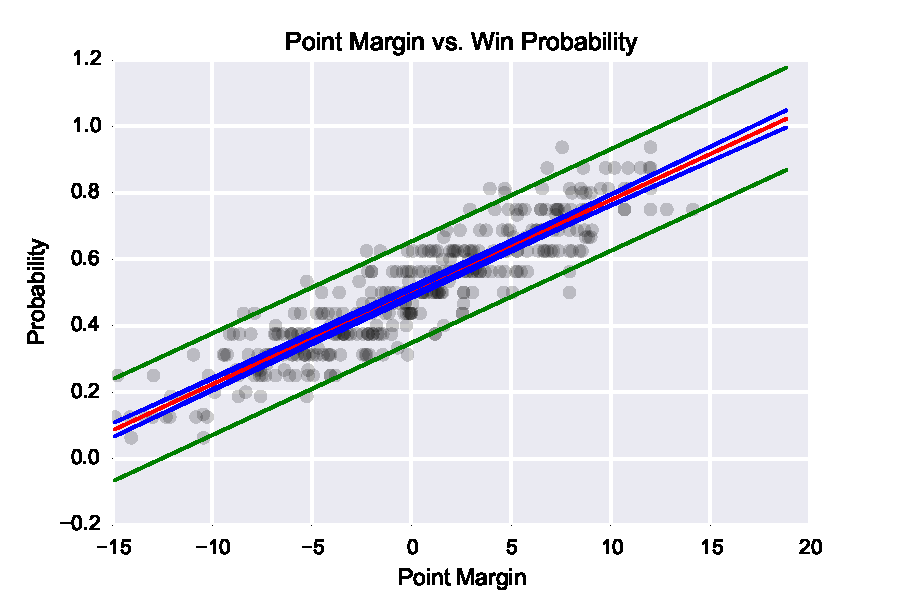
\includegraphics[scale = 1]{MarginWinProb.pdf}
\end{center}

\indent This plot shows the very strong, positive linear relationship between expected point margin and winning percentage. These figures are calculated per team, per season over the 2002 - 2012 seasons in the NFL. Expected point margin is an important variable to examine when making a fourth down decision in the early to mid-stages of the game because of this relationship. This is an observational exploratory data analysis so causal relationships cannot be proved, however the association is worth noting.\\    
\indent Expected point margin is an important factor in a fourth down judgment call, but there are spots in the game when this obviously should not be the case. The first oddity and solvable problem are decisions in the fourth quarter. Obviously, it would not be wise to go for a fourth down only because the expected point margin is greater for that particular decision. In the fourth quarter, coaches and management must be playing the score, as well as the clock. Because our model does not account for the clock, one should not use our model for many fourth quarter situations. If you are interested about decisions in the fourth quarter, you can read about a win percentage model, which is a model only relevant for fourth quarter situations. This is because not enough teams go it on fourth downs earlier in the game. Our model is purely constructed to give optimal decisions in the first three quarters (excluding the last four minutes before half), when your team likely has a greater chance of winning if the expected point margin increases in your favor. \\
\indent One challenging aspect of our task was to measure the expected point spread on the same scale. You might be asking, what does that mean? We think an example is the most efficient way we can communicate this. For this example, consider the team making the fourth down determination, Team A, and the opposing team, Team B. If Team A decides to punt, Team B has the ball next possession. If Team A decides to go for it, and they convert, Team A has the ball the next possession. At the end of these drives in one situation Team A possesses the ball, and in the other Team B possesses the ball.\\
\indent Obviously, this is a problem that must be corrected. In order to account for this complex issue, we decided to calculate the expected point spread difference until Team A re-obtains possession of the ball after the end of their current drive. So, for example, if Team A chooses to punt, their drive ends. Then, Team B has one drive until Team A re-obtains possession of the ball. If Team A decides to go for it, two things can happen, they can either convert or not convert. If Team A converts, they maintain possession of the ball on their current drive. After their drive ends, Team B has a drive. After both of these drives are done, Team A regains possession of the ball, thereby ending the observation. If Team A does not convert, they give Team B possession of the ball where they tried the conversion. Then, Team B has a drive until Team A re-obtains possession of the ball, ending the observation. If Team A kicks a field goal, they can again either convert or not convert. In each of these cases, after the field goal attempt, Team A's possession is over. Team B possesses the ball and drives down the field. After this drive, Team A re-obtains possession of the ball, which ends the observation. \\ 
\indent One can see that now our observations are all measuring the same thing: the expected point marginal difference given a decision. This is pivotal because it allows us to compare the three decisions directly. It is hard to think about the possibilities of the outcomes of these decisions in an NFL game because they are complex and multi-dimensional, but our model creates a way to make comparisons that are valid and direct. \\
\indent So, let's assume Team A is in a fourth down predicament; they are facing a fourth and one from the 50 yard-line. The following numbers are reasonable, but they are not calculated from our model. The example is to give an idea how a decision is made. Given Team A decides to punt, Team B is expected to score 1.7 points before they give possession back to Team A. The point spread for Team A is -1.7, because they are 1.7 points worse off than before. If Team A instead chooses to go for it, let's assume they convert with probability .7. Given Team A converts, Team A is expected to score 3 points on their current drive. After Team A's conversion and drive, Team B is expected to score 2 points before Team A re-obtains possession. Given Team A does not convert, Team B is expected to score 3 points before Team A re-obtains possession. Then Team A is on average $(.7(3 - 2) + .3(-3) = -.2)$ $.2$ points worse off than before. If Team A decides to kick a field goal, let's assume the probability of conversion is .01. If Team A converts they score 3 points, then after the conversion Team B is expected to score 2 points before giving the ball back to Team A. If Team A does not convert, Team B is expected to score 3.5 points before Team A gains possession again. Then Team A is on average $(.01(3 - 2) + .99(-3.5) = -3.455)$ $3.455$ points worse off than before. From our expected spread calculations, Team A should go for it because the point spread, although negative, is better if they choose this decision than either punt or field goal.   \\
\indent In calculating these expected point spread changes, one must be aware of a few implementation decisions we made. First, for punts, the calculation is the negative expected number of points Team B will score on their next drive given Team A punted from a certain yard-line. The calculation is not the expected number of points given Team B starts 38 yards (net punt average) further down the field. We feel our approximation is solid because it factors in blocked punts, and punts that are far away from the average of 38 yards. Second, if the decision was to go for it, we assumed several things. If Team A converted the first down, we assumed Team A would maintain possession of the ball at the position of the first down marker. If Team A did not convert the first down, we assumed Team B would obtain possession of the ball at the yard-line where Team A attempted the first down. Obviously, this is not usually the case. On fourth and 1 for instance, Team A has a possibility of gaining 3 yards, or 10 yards, or maybe even scoring a touchdown. And, if they do not convert, Team B has the possibility of sacking the quarterback or intercepting a pass which means Team B is not necessarily going to start their drive from the position Team A attempted the first down. These two assumptions are not always true, but at least they pull in different directions. If Team A converts, then we are underestimating their expected points. In our example, Team A might score on average 3.5 points instead of 3 because Team A is maintaining their drive from the 49 yard-line or better, not exactly the 49 yard-line. If Team A does not convert, maybe Team B scores 3.5 points their next drive instead of 3. Because Team B is not necessarily starting their drive from the 50. They could have turned Team A over and returned the ball 30 yards thus increasing the expected points they would score. These are valid concerns that one must be aware of, but because they are happening in opposite directions, hopefully our results are not very biased. Controlling for these factors to improve our prediction estimates could and should be done in later research. The only problem not accounted for in field goal try's was that we did not factor in the probability of blocked field goals into our calculation. This happens very rarely so we figured the difference in expected point spread would be negligible. However, it is a good idea to note that the expected values for the field goal decision are most likely just a little too high. \\
\indent After researching and deciding on our implementation method, we needed a way to evaluate the prowess of the offensive and defensive units of a certain team. We decided to focus on number of points scored and number of points surrendered throughout the course of a season. The higher the number of points scored in a season, the better the offense. The fewer points allowed in a season, the better the defense. There are certainly other variables one can use to assess the ability of an offensive and defensive unit, but we felt this simple method was good enough. After calculating these values we plotted each of the 32 teams offensive and defensive trends in the following plots. 

\begin{center}
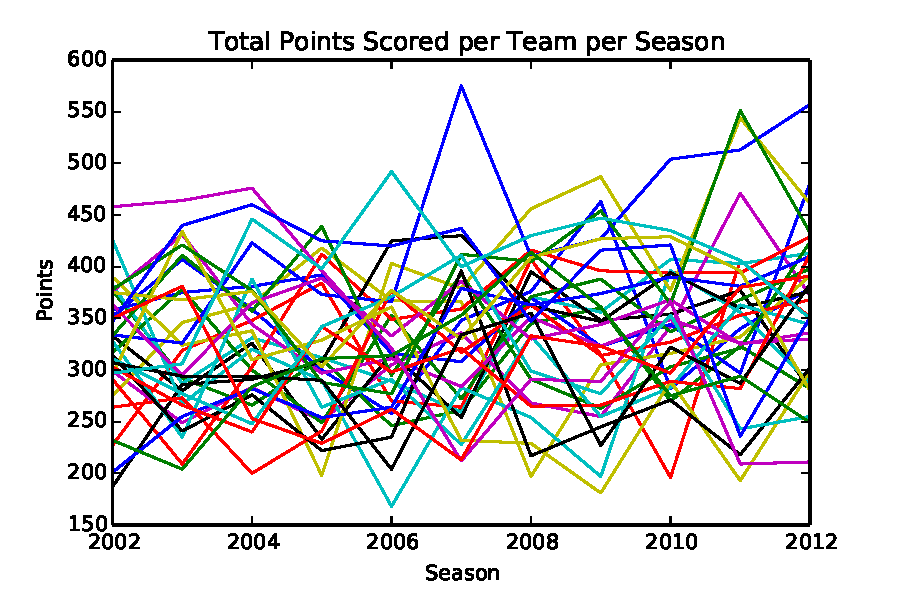
\includegraphics[scale = 1]{OffTeamperSeason.pdf}
\end{center}


\begin{center}
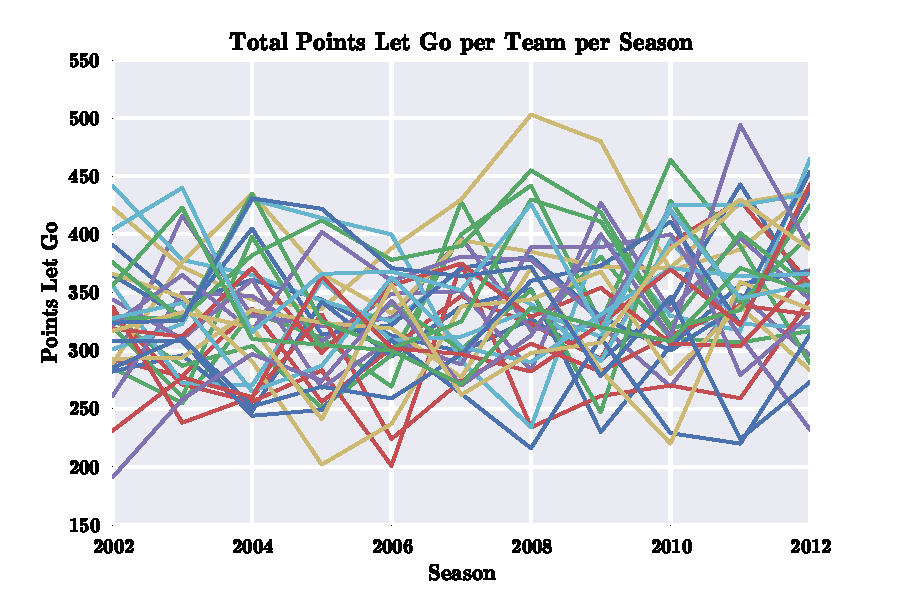
\includegraphics[scale = 1]{DefTeamperSeason.pdf}
\end{center}


\indent There is only one clear takeaway from this plot: it isn't clear at all. The teams offensive and defensive abilites are changing a lot for the 11 seasons we researched. For example, the San Francisco 49ers went from one of the worst defenses in the league in 2007 to one of the best in 2012.\\
\vspace{10 mm}

\indent This messy time series plot changed our focus. We chose to rank the teams 1 to 32 (1 = best, 32 = worst) on offense and defense every season, and make the rankings our new ``teams". So, for instance, if the Green Bay Packers scored the most points in the year 2002, they would have the number one ranked offense in that season. Then, if the New England Patriots scored the most points in 2003, they would have the number one ranked offense for that season. So, essentially, the Green Bay Packers 2002 offense and the New England Patriots 2003 offense are the same because they were both number 1 ranked. We did this for all 32 ranks in the 11 seasons for both offense and defense. After, we made this correction our plots of ranking and years look much better for both offense and defense. 

\vspace{30 mm}

\begin{center}
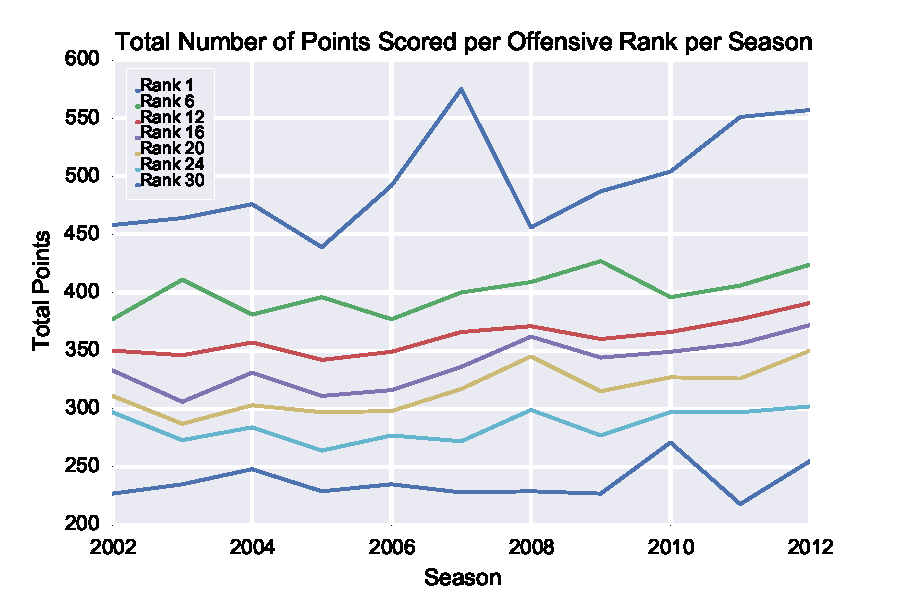
\includegraphics[scale = 1]{OffRankperSeason.pdf}
\end{center}


\begin{center}
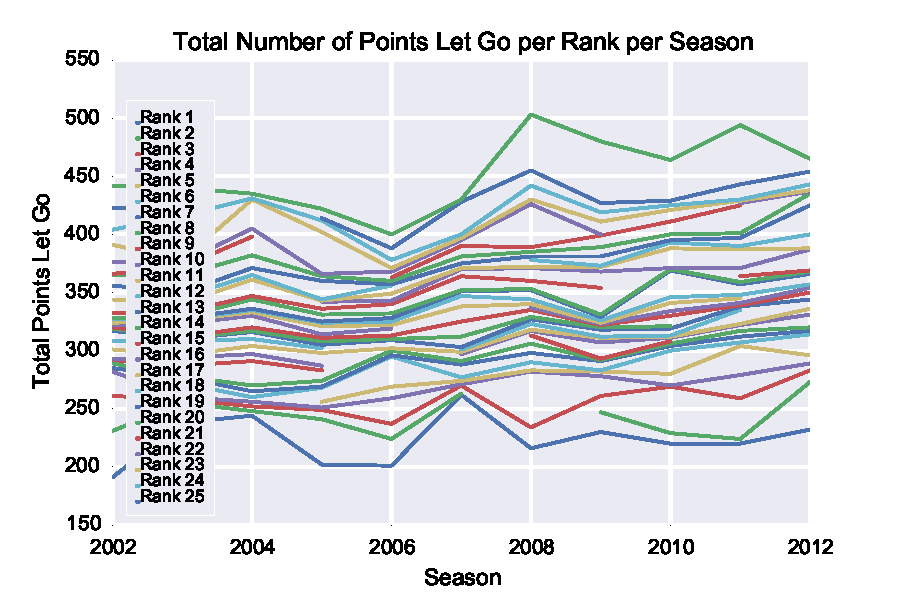
\includegraphics[scale = 1]{DefRankperSeason.pdf}
\end{center}

\vspace{30 mm}

\indent The previous two graphs show the top four and bottom two teams are many times outliers in particular seasons. Many times the difference between these outlying teams expected points is greater than the difference for the teams in the middle. Because of this we created dummy variables, one for those teams ranked 31 and 32, and one for those teams ranked 5 - 30 (for both offense and defense). The dummy variable between 5 and 30 are linearly related so we multiply this linear factor by the 5 - 30 dummy. However, teams 31 and 32 are close enough that we simply create a 0 - 1 dummy variable. Because of these dummies, our models are estimated in comparison to offenses and defenses ranked 1 - 4. Notice from the plots, that number one ranked offenses are at the top where as number one ranked defenses are at the bottom. The reasoning is simple; the best offenses score the most number of points and the best defenses give up the fewest. \\

\newpage

\indent After finding all of the values for our explanatory variables (yard-line and yards to go given in the dataset), we can start estimating the probability of conversions, an essential piece of the expected point spread calculation. A conversion or non-conversion happens in two of the three scenarios: field goal, or go for a first down. Obviously, the outcome in each of these estimations is binary. When attempting a field goal, either the kick is good or no good. Likewise, when attempting the first down, either the team converts the first or does not convert. Because our response is binary for each of these decisions, we will use the logistic regression model. A very popular model when there is a binary response. The assumptions of the model seem satisfied: our response is clearly binary, and the explanatory variables seem independent. Therefore, we ran our models and computed 95 percent confidence intervals for given situations. \\
\indent The following table gives the results of our logistic model in determining the probability of converting a field goal. \\

\vspace{20 mm}


\begin{center}
\Large \bf Logistic - Field Goal \\
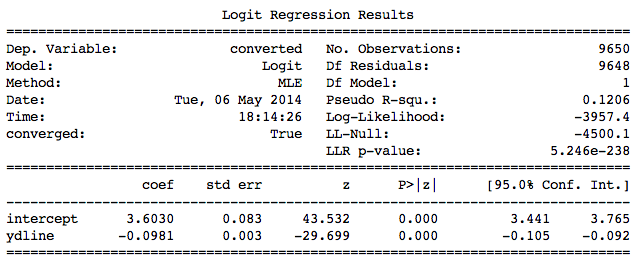
\includegraphics[scale = .75]{Table_FieldGoal.png}
\end{center}

\newpage

\indent From the graph below, it is obvious that the probability of a conversion attempt is very close to 1 when it is a short kick (a kick with 0 yards to your goal-line, or a 17 yard field goal). This is not surprising at all, because extra point attempts are from 20 yards away and kickers make close to 100 percent of extra point attempts (1). However, as one gets further and further away it may surprise some people that the percentage decrease for very long field goal attempts is not more drastic. When you have 50 yards to go (a 67-yard field goal) our model predicts about a 20 percent conversion rate. This obviously is too high; no one has ever converted a field goal of longer than 63 yards. There are three major reasons why these probabilities are clearly inflated. Firstly, only the kickers with huge legs like Sebastian Janikowski kick field goals greater than 60 yards. Secondly, they usually kick these field goals in nice weather, possibly in Denver, where the altitude might give a kicker 5 or so yards of added range. And lastly, 67 yard field goals are not in our data set. The logistic regression model does not accurately predict response values when the explanatory variables are outside of the range in the dataset. For these reasons, deep field goal probability calculations are too high. From about the 40 yard-line and in, however, our results are more than believable. But, field goal success rate also depends on your kicker and on the weather. These results average over all kickers and different weather. If you are kicking in snow, or have a terrible or great kicker, the coach should adjust the expected value of kicking a field goal accordingly.

\begin{center}
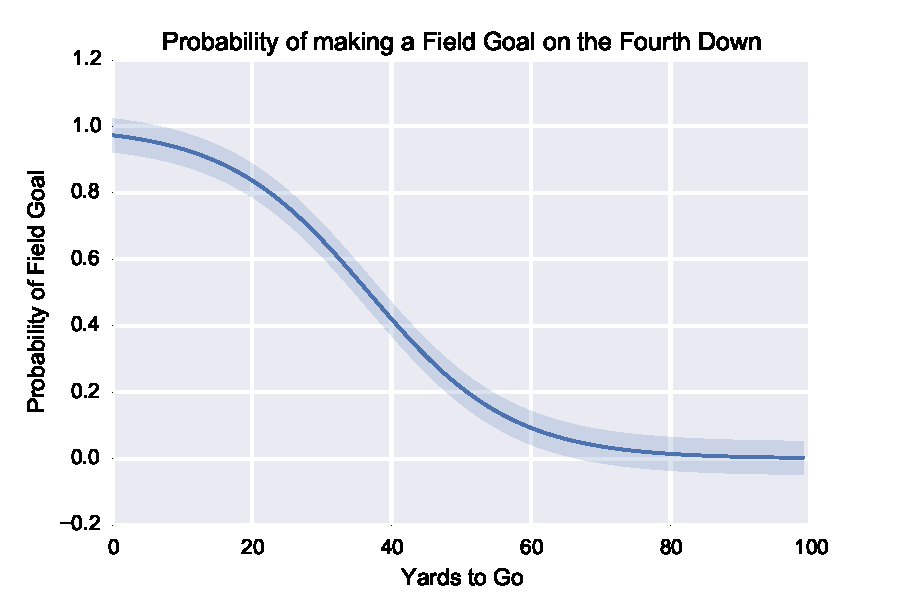
\includegraphics[scale = 1]{fieldgoalprob.pdf}
\end{center}

\newpage

\indent From our data set, we decided not to use fourth down plays to model our fourth down conversion rates for one clear reason. The vast majority of fourth down plays are not the ones we want to model. Because of the conventional wisdom in the NFL, a huge majority of fourth down plays where the team decided to go for it happened in the fourth quarter, or with 4 minutes or less left in the second quarter. These are not the plays we want modeled, and they are very different to the plays we want modeled. Many times defenses will be playing what is known as ``prevent" defense in these particular situations. This essentially means that the defense would allow a 5 or 10 yard play, in order to prevent the deep pass. Why? Becuase, for instance, if you're up by 10 with 2 minutes left a 10 yard completion and conversion on fourth down does not hurt too much. However, a deep touchdown now creates a real dilemma. Becuase of situations like these, using these observations would inflate our fourth down probabilities which we our trying to model in quarters 1 to 3 (except 4 or less minutes in the second quarter). \\
\indent So, where does that leave us. If we can't use fourth down plays from our dataset to estimate fourth down conversion rates, what can we use? Well, because of the current nature of the NFL, third downs are very similar to the fourth downs we want modeled. Offenses understand that if they do not convert on third down, they will almost always punt on fourth down. The desperation of third down is pretty similar to that of fourth down. Therefore, we can use third down plays to estimate fourth down conversion rates in the first three quarters. However, several third down plays should be extracted. Third and long (10 or greater) in which a team decides to run we extracted because they would bias our results. Usually, on these plays coaches are not attempting to convert the first down, but rather not throw an interception or give their punter room to punt if they're backed up on the field. Obviously, if it was fourth down, teams would not be so conservative. \\
\indent After using third downs to model fourth down plays, we know that the probability of a fourth down conversion should change depending on the strength of the deciding teams' offense, the opposing teams� defense, the number of yards to go for a first down, and the field position.  From our model, you can see that as the yards to go increases the probability decreases. Also, the better the offense is in comparison to the defense, the probability of conversion increases. We also turned yard-line into a categorical variable. This categorical variable indicates whether the fourth down conversion is 0 - 10, 10 - 30, 30 - 50, 50 - 70, 70 - 90, or 90 - 100 yards from the goal-line. You can see from these probabilities that the conversion rate from 0-10 yards is lowest (the base for the yard-line dummy variable in the logistic model) because all the yard-line coefficients are positive. Then, as one might expect, the conversion rate, if you have greater than 90 yards to the goal-line, is low in relation to the other yard-lines as well because teams are nervous about safety possibilities and other factors.

\newpage

The following table gives the results of our logistic model in determining the probability of converting a first down

\vspace{30 mm}

\begin{center}
\Large \bf Logistic - Go For It \\
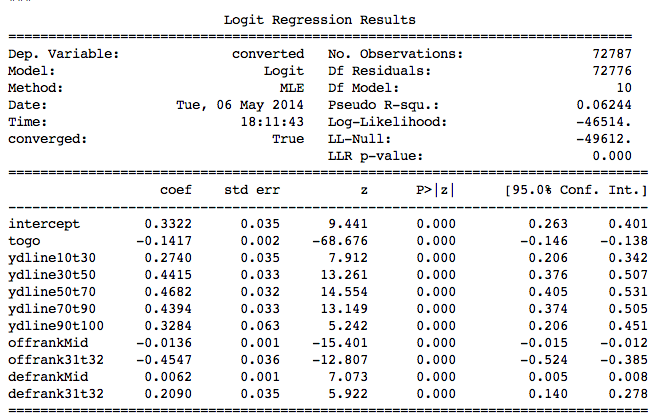
\includegraphics[scale = .75]{Table_GoForIt.png}
\end{center}

\newpage



\begin{center}
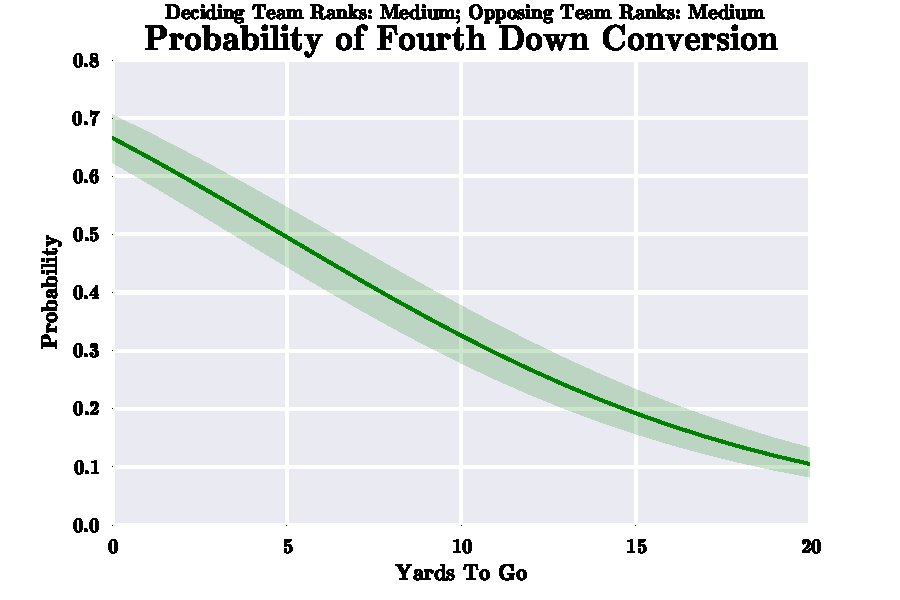
\includegraphics[scale = 1]{gfi_15_15_prob.pdf}
\end{center}

\vspace{30 mm}

\indent The graph above assumes a medium ranked deciding team's offense and opposing team's defense (both 15th), and that the decision occurs between the 50 and 70 yard-line. Given these two ranks, this graph plots the effect of the number of yards to go on conversion rates. You can clearly see that the probability of conversion is about 68 percent with one or fewer yards to go, and steadily goes down to about 10 percent with 20 yards to go. These numbers are pretty consistent with the numbers published in a few papers about league average (2). 

\newpage


\begin{center}
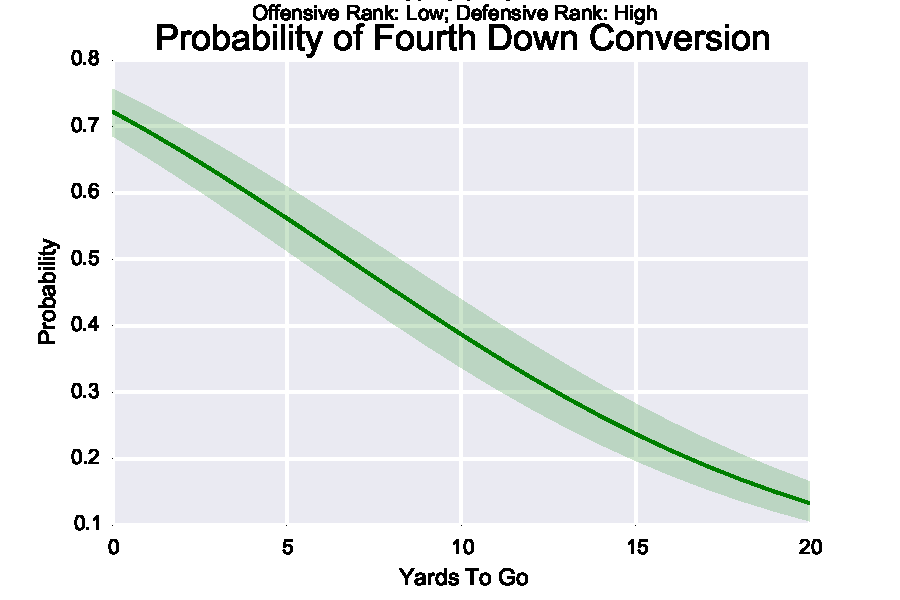
\includegraphics[scale = 1]{gfi_1_25_prob.pdf}
\end{center}

\vspace{30 mm}

\indent If the yard-line remains the same, but the deciding team's offensive rank is high (5th) and the opposing team's defensive rank is low (25th) one can see that the probability increases slightly when comparing across yards to go from the previous plot. Instead of the graph steadily decreasing from about 68 percent to 10 percent (0 to 20 yards away), the probabilities range from 72 percent to 14 percent. The confidence intervals slightly overlap, but the slightly higher probabilites intuitively make sense. Better offenses convert at higher rates, and lower ranked defenses give up the conversion at higher rates.

\newpage

\indent The expected number of points is calculated by multiplying the possible outcomes of a drive by the point values given those outcomes. In each drive there are five possible outcomes: a touchdown, field goal, no points by the offense, a safety, or a touchdown by the defense. These numbers are multiplied by the points of each outcome: 7, 3, 0, -2, and -7 respectively. For the model, we assume every touchdown is 7 points (not 6 or 8). This is true the vast majority of the time. In order to estimate the probabilities of these outcomes we decided to use a multinomial logistic regression model. A multinomial model is used for a categorical response variable (here five categories) when the explanatory variables are independent. Here, the explanatory variables for our model are the offensive rank of Team A (the deciding team) and the defensive rank of Team B (the opposing team)  as well as the starting field position. The assumption of independence seems reasonable. 

\begin{center}
\Large \bf Multinomial Logistic - Regular
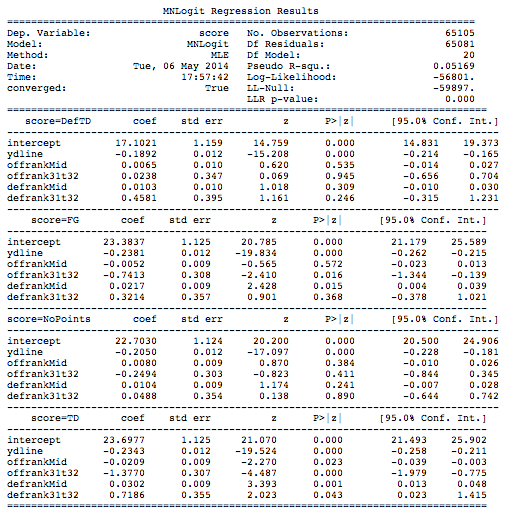
\includegraphics[scale = .75]{Table_ScoreLogit.png}
\end{center}

\newpage

In our project, a model is also used to determine the number of points for Team B given Team A punts from a certain yard-line. This is exactly the same as the last model except the explanatory variables are Team B's offense, Team A's defense, and ``starting field position" becomes ``punt yard-line by Team A".

\vspace{30 mm}

\begin{center}
\Large \bf Multinomial Logistic - Punt
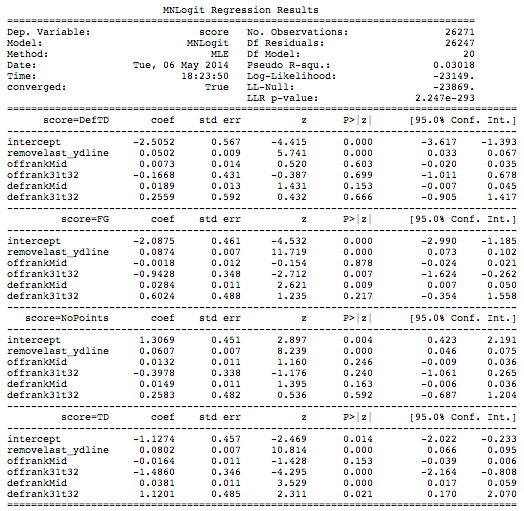
\includegraphics[scale = .75]{Table_PuntLogit.png}
\end{center}

\newpage

\indent If you notice, the expected spread calculations can get complicated if for instance Team A (the deciding team) punts and gets a defensive touchdown on Team B's next drive. In this scenario Team B would get the ball back and the observation would not be over until Team A re-obtained possession of the ball on offense. So, if this happens our model multiplies the probability of a defensive touchdown by 7 minus the expected number of points of Team B's next drive. You notice that this is a recursive relationship. If Team B gets the ball back they can again give up another defensive touchdown and repeat the process. Luckily, the probability of a defensive touchdown is so low regardless of field position that the expected point margin converges quickly. Something similar happens if Team A chooses to go for it and converts, then gives up a safety. If this happens, again our model recursively calculates Team B's next drive until Team A re-obtains possession of the ball on offense. Luckily, both of these probabilities are so low in any scenario that this does not have a big effect on our expected point spread calculations. \\ 
\indent From the multinomial and logistic regressions, we can now calculate the effect of point spread for each decision. \\
\indent Let $Points_{A}$ and $Points_{B}$ be the number of points Team A and Team B will score respectively. Let $Punt$, $Field Goal$, and $Go For It$ be the events that Team A punts, attempts a field goal and goes for the 1st down given they are on their fourth down respectively. Let $S_{f}$ and $S_{g}$ be the events that Team A converts a field goal and converts a first down respectively. Then let

\begin{gather*}
P = E[Points_{A} | Punt] \\
G = E[Points_{A}|\text{Go For It}] = E[Points_{A}| S_{g}]P(S_{g}) - E[Points_{B}|S_{g}^c]P(S_{g}^c)\\
F = E[Points_{A}|\text{Field Goal}] = E[Points_{A}| S_{f}]P(S_{f}) - E[Points_{B}|S_{f}^c]P(S_{f}^c)\\
\end{gather*}
Then Decision $= argmax\{P, G, F\}$ \\
\indent For the expectation of point spread given you punt, we use the multinomial logistic regression model based on punts. This model outputs the probabilites of certain outcomes for Team B's next drive. Once these probabilities are obtained we can multiply each one by that specific point outcome. For example:
\begin{gather*}
P = 7*Pr(\text{Team B Touchdown}) + 3*Pr(\text{Team B Made Field Goal}) \\  - 2*Pr(Safety) - (7 - E[\text{Points For Team B} | \text{Team A Kickoffs}])*Pr(\text{Defensive Touchdown})
\end{gather*}
\indent Remember that if Team A records a defensive touchdown against Team B, Team B will get the ball back so the observation does not end. Therefore, the Pr(Defensive Touchdown) is multiplied by 7 - E[Points For Team B | Team A Kickoffs]. This expected value is calculated from the regular multinomial logistic regression model with Team B on offense, Team A on defense, and 80 yards to go for a touchdown. We will assume Team B starts from the 80 yard-line because often Team A will kick a touchback after they score. \\
\indent Point spread given you go for it is a little more complex. First of all the probability of converting or not converting the first down is estimated from the basic logistic regression model discussed earlier. Once we have these two probabilities, we can find the expected point values for both situations using the regular multinomial logistic regression model. If you convert the first down, we assume your new yard-line is where the first down marker was before deciding to go for it. Given this new yard-line Team A's current drive will result in certain probabilities of scoring different point values based on Team A on offense, and Team B on defense. We can calculate the expected number of points in a similar fashion as the punt equation: 
\begin{gather*}
E[Points_{A}|  \text{Convert 1st Down}] = 7*Pr(\text{Team A Touchdown}) + 3*Pr(\text{Team A Made Field Goal}) \\ - 2*Pr(\text{Team B Safety})  - 7*Pr(\text{Team B Defensive Touchdown})
\end{gather*}
\indent Now, we have the probability Team A scores or does not score after a successful fourth down conversion. $Pr(score) = Pr(Touchdown) + Pr(Made Field Goal)$. The probability of not scoring is $P(No Score)$ or one minus the sum of all other probabilities. So if Team A scores we use the same multinomial logistic probabilities with Team B's offense having to travel 80 yards against Team A's defense. If Team A does not score, we estimate the starting yard-line for Team B by using a linear regression equation. This method gave adequate, sensible results. So, if Team A converts the first down, but does not score, then Team B scores by multiplying the probabilities of all outcomes by the outcome values given this regression calculated yard-line with Team B on offense, and Team A on defense. If the fourth down attempt is not converted, then Team B will simply get the ball at the yard-line Team A was trying to convert from. Then we will use the regular multinomial logistic regression equation with Team B on offense, Team A on defense, and this yard-line. Also, keep in mind that in order to remain consistent, defensive touchdowns and safeties were accounted for so Team A always had possession at the end of the observation. \\
\indent If you choose to kick a field goal, the expected value calculations are again based on a logistic regression model and the regular multinomial logistic regression model. The logistic regression model based on field goal conversion is used to determine the probability of a successful field goal given a kick is from a certain yard-line. Once the probabilities of a made field goal and a missed field goal are obtained, the calculations for expected values are relatively straightforward. If the field goal by Team A is made, Team B gets the ball after the kickoff. Like the punt and go for it expected spread calculations, Team B is assumed to need 80 yards to score a touchdown. So, the regular multinomial logistic regression equation can be used to obtain the probabilities and calculate the expected value in the same way as before. If the kick by Team A is no good, Team B takes over possession of the ball at the attempt of the kick (yard-line plus 7 yards). Again, the regular multinomial logistic regression equation can be used with Team B on offense, Team A on defense, and this new yard-line. \\ 
\indent We also computed a confidence interval for each of the three scenarios by taking each of the lower bounds and upper bounds of the combined intervals and adding them together. Because of the complexities in this calculation the estimated line is not in the middle of the confidence interval. Also, this interval is technically greater than 95 percent because we are combining other 95 percent confidence intervals. \\
\indent The next plots illustrate how the yard-line affects the optimal decision, with given offensive and defensive ranks of both the team making the decision and the opposing team (all ranks around 15). In the first plot the optimal decision is to kick a field goal regardless of the number of yards to go. However, with less than one yard to go the confidence intervals overlap which means it may be optimal to go for the first down. The coach should make the final decision if the intervals overlap. On the 50 yard-line, with the same rankings, the optimal decision changes in a pretty major way. Now, the graph indicates that a team should go for the first down on fourth and less than 6, between 6 and 12 yards either punt or go for it, and past 12 yards punt. With 80 yards to the goal-line, a team�s optimal decision is to go for it on fourth and less than 3, either punt or go for it between 3 and 9 yards to go, and punt the ball if there are more than 9 yards to go for a first. 

\newpage


\begin{center}
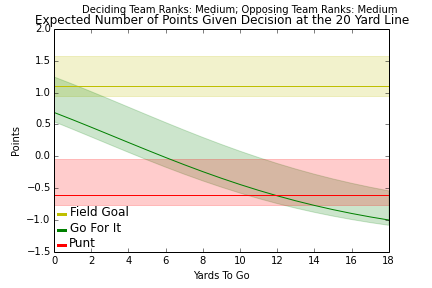
\includegraphics[scale = .7]{Decision2015161516.png}
\end{center}


\begin{center}
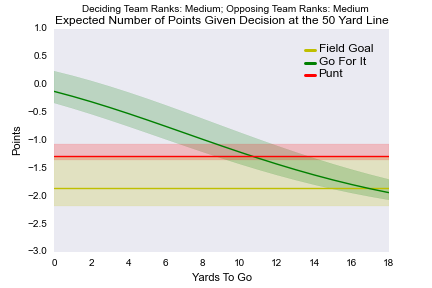
\includegraphics[scale = .7]{Decision5015161516.png}
\end{center}



\begin{center}
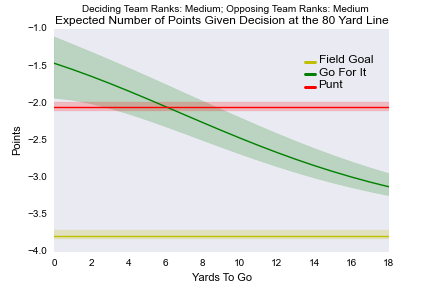
\includegraphics[scale = .7]{Decision8015161516.png}
\end{center}

\newpage

\indent This progression is common to all offensive and defensive ranks. The 3 charts below paint the picture for the optimal decision for every position on the field and any fourth down situation less than 20 yards to go for certain rankings of the offensive and defensive units of both teams. If the team making the decision has a high ranking offense and defense, and the opposing team has a low ranking offense and defense, the optimal decision in many circumstances is to go for it. Our calculations project that it is optimal to attempt the first down anywhere on the field which is fourth and less than 2. The optimal decision map also indicates that you should go for it from about fourth and 15 from the 50, as well as fourth and 7 with 97 yards to the goal-line. These numbers are obviously very surprising, but they are partially high because of the unusually large difference between the teams� rankings.

\vspace{30 mm}

\begin{center}
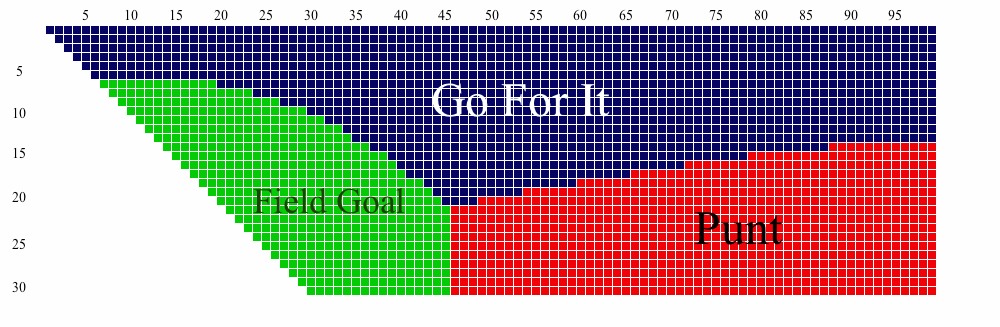
\includegraphics[scale = .5]{GridBlock112525.png}
\end{center}

\newpage 

\indent If the teams are ranked evenly for both offense and defense then our map become more conservative. Now, the map indicates that a team should attempt the first down conversion from fourth and 8 with 50 yards to the goal-line and fourth and 4 with 96 yards to the goal-line. 

\vspace{5 mm}

\begin{center}
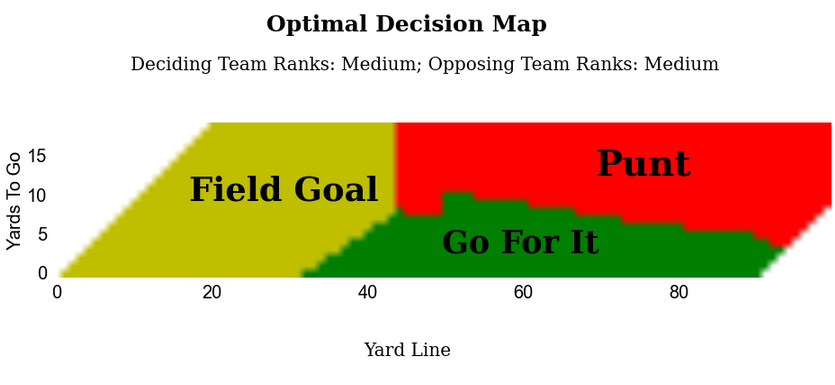
\includegraphics[scale = .5]{GridBlock15151515.png}
\end{center}

\indent The optimal decision map becomes even more conservative when the team making the decision is weak on both offense and defense, and the opposing team is strong offensively and defensively. Now, the decision map�s optimal values are to go for the first down on fourth and four from the 50, and go for it on fourth and one with 91 yards to the goal-line.

\vspace{5 mm}

\begin{center}
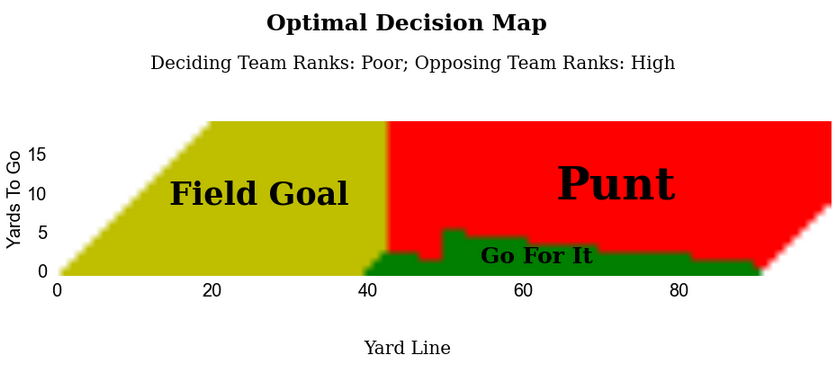
\includegraphics[scale = .5]{GridBlock252511.png}
\end{center}

\newpage

\indent Obviously, the ranking of both teams� offense and defense have an enormous impact on the optimal decision. For a high ranking offense, a coach should go for it much more often given other rankings remain constant.

\begin{center}
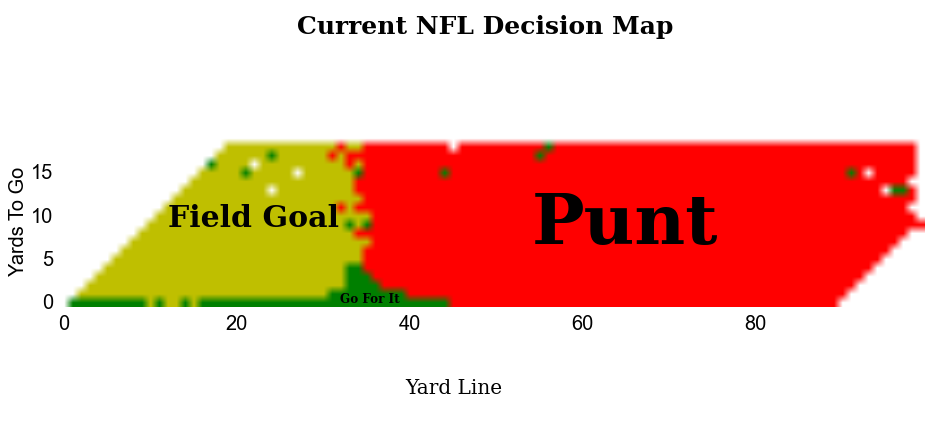
\includegraphics[scale = .5]{GridBlockActual.png}
\end{center}

\indent The dramatic changes in these plots purely due to teams� offensive and defensive ranks are interesting, but how does the overall trend compare to current NFL fourth down decision making may be a better question? The above plot shows the decisions coaches and upper management have made over these 11 seasons. When comparing the maps, there are stark differences from our previous three optimal decision maps. The first major difference is that teams rarely go for it. In fact, anywhere past the 45 yard-line the decision most often made in nearly every scenario (combination of yard-line and yards to go) is to punt. One other noticeable feature is that our earlier plots had kickers going for field goal attempts from much larger distances. Once again, this value is heavily inflated because of the higher than should be conversion rate of deep attempts. \\
\indent Our analysis should not convince you that the results we obtained are perfect. The data used in our analysis is observational, and there is no way to prove causality. Therefore, coaches� deep level of knowledge of the game should still play a major role in determining the fourth down decision. But, their football expertise along with an understanding of the estimated expected values could help guide their decision under uncertainty. The clear difference between our logical model and the current NFL's usual decision is obvious. We still would not recommend going for a first down on fourth and seven from your own 3 yard-line. However, our process makes intuitive and mathematical sense. And the optimal decision is most likely somewhere in the middle. Obviously, giving up possession of the ball by punting has a much greater negative effect than teams currently realize. \\
\indent The model could be improved, and the assumptions fortified given additional time. But, this is a good start in showing that fourth down decision making in the NFL is off base. With the rise of data analytics in sports, it will be interesting to see if there is a change in fourth down philosophy from its traditional logic to a more modern approach. We believe the teams that adopt this strategy will have a clear advantage over their opponents.

\end{document}